\documentclass[aspectratio=1610,12pt]{beamer}

\usepackage{comment}
%\usepackage[utf8]{inputenx} % For æ, ø, å
%\usepackage[T1]{fontenc}
\usepackage[english]{babel}          % Automatic translations
%\usepackage{fancyvrb}
\usepackage{minted}
\usepackage{csquotes}       % Quotation marks
\usepackage{microtype}      % Improved typography
\usepackage{amssymb}        % Mathematical symbols
\usepackage{mathtools}      % Mathematical symbols
%\usepackage{anyfontsize}
\usepackage{tikz}
%\usepackage{svg}

\usepackage{booktabs}

\usepackage{bussproofs}
\EnableBpAbbreviations

\graphicspath{{./pictures/}}

\usetheme{Dresden}
\usecolortheme{spruce}

\errorcontextlines=10000
\maxdimen=16383.99999pt
\pdfobjcompresslevel=0
%links
\usepackage{hyperref}

%seitennummer
\setbeamertemplate{page number in head/foot}[totalframenumber]

%Ausblenden der zweiten Kopfzeile
\usepackage{soul}
\makeatletter
\let\HL\hl
\renewcommand\hl{%
  \let\set@color\beamerorig@set@color%
  \let\reset@color\beamerorig@reset@color%
  \HL}
\makeatother

\defbeamertemplate*{headline}{miniframes theme no subsection}
{%beamer template
  \begin{beamercolorbox}[colsep=1.5pt]{upper separation line head}
  \end{beamercolorbox}
  \begin{beamercolorbox}{section in head/foot}
    \vskip2pt\insertnavigation{\paperwidth}\vskip2pt
  \end{beamercolorbox}%
  \begin{beamercolorbox}[colsep=1.5pt]{lower separation line head}
  \end{beamercolorbox}
}

\setbeamertemplate{footline}{%
  \leavevmode%
  \hbox{%
    \begin{beamercolorbox}[wd=.5\paperwidth,ht=3.2ex,dp=1.8ex,left]{author in head/foot}% Adjusted height and depth for margin
      \usebeamerfont{author in head/foot}\hspace*{2ex}\insertshortauthor
    \end{beamercolorbox}%
    \begin{beamercolorbox}[wd=.5\paperwidth,ht=3.2ex,dp=1.8ex,right]{title in head/foot}% Adjusted height and depth for margin
      \usebeamerfont{title in head/foot}\insertframenumber{} / \inserttotalframenumber\hspace*{2ex}
    \end{beamercolorbox}}%
  \vskip0pt%
}

\setbeamertemplate{footline}[miniframes no subsection]

%sources
\usepackage[absolute,overlay]{textpos}
\setbeamercolor{framesource}{fg=gray}
\setbeamerfont{framesource}{size=\tiny}
\newcommand{\source}[1]{\begin{textblock*}{15cm}(0.4cm,8.8cm)
    \begin{beamercolorbox}[ht=0.5cm,left]{framesource}
      \usebeamerfont{framesource}\usebeamercolor[fg]{framesource} {#1}
    \end{beamercolorbox}
  \end{textblock*}}

\definecolor{UBCblue}{rgb}{0.04706, 0.13725, 0.26667} % UBC Blue (primary)
\definecolor{UBCgrey}{rgb}{0.3686, 0.5255, 0.6235} % UBC Grey (secondary)
% define color with hex #00883A
\definecolor{LMUmain}{HTML}{00883A}
\definecolor{LMUsec}{HTML}{00F56A}
\definecolor{LMUacc}{HTML}{8C4091}

\setbeamercolor{palette primary}{bg=white,fg=LMUmain}
\setbeamercolor{palette secondary}{bg=LMUmain,fg=white}
\setbeamercolor{palette tertiary}{bg=LMUmain,fg=white}
\setbeamercolor{palette quaternary}{bg=LMUmain,fg=white}
\setbeamercolor{structure}{fg=LMUmain} % itemize, enumerate, etc
\setbeamercolor{section in toc}{fg=LMUmain} % TOC sections

\setbeamercolor{block body alerted}{bg=alerted text.fg!10}
\setbeamercolor{block title alerted}{bg=alerted text.fg!20}
%\setbeamercolor{block body}{bg=structure!10}
%\setbeamercolor{block title}{bg=structure!20}
\setbeamercolor{block body example}{bg=LMUacc!10}
\setbeamercolor{block title example}{bg=LMUacc!20}


\usepackage{hyperref}
\usepackage{tikz}
\usepackage{qrcode}
\usepackage{pgfplots}
\usepackage{pgfplotstable}
\usepackage{svg}
\usepackage{minted}
\usetikzlibrary{positioning}
\usetikzlibrary{shapes.symbols}
\usetikzlibrary{shapes.multipart}
%\usepackage[sfmath]{kpfonts}
%\usetikzlibrary{external}
%\tikzexternalize[prefix=tikz/]
\beamertemplatenavigationsymbolsempty


\author{Ruben Triwari}
\title{Comparing Natural Language Embeddings for Libc Functions as Rich Labels}
\subtitle{Bachelor defense}
\institute{Ludwig Maximilian University Munich}
\date{19, February 2025}

\newcommand*{\qt}[1]{'#1'}
\newcommand*{\p}{^\prime}
\newcommand*{\as}{\;}% "apply-space" for λ-calc
\newcommand*{\la}{\lambda}
\newcommand*{\N}{\mathbb{N}}

\newcommand*{\sps}{\mathcal}
\newcommand*{\tsc}{\textsc}
\newcommand*{\opn}{\operatorname}

\newcommand{\cn}[2]{\textcolor{#1}{#2}}%color next (element)
\newcommand*{\C}{\mathbf{C}}
\definecolor{c1}{RGB}{189, 57, 57}
\definecolor{c2}{RGB}{57, 155, 163}
\definecolor{c3}{RGB}{16, 14, 77}

\definecolor{SkyBlue}{RGB}{135, 206, 235}
\definecolor{CrimsonRed}{RGB}{220, 20, 60}
\definecolor{ForestGreen}{RGB}{34, 139, 34}
\definecolor{Goldenrod}{RGB}{218, 165, 32}
\definecolor{DeepPurple}{RGB}{75, 0, 130}
\definecolor{Coral}{RGB}{255, 127, 80}
\definecolor{Teal}{RGB}{0, 128, 128}
\definecolor{Lavender}{RGB}{230, 230, 250}
\definecolor{Amber}{RGB}{255, 191, 0}
\definecolor{SlateGray}{RGB}{112, 128, 144}

\definecolor{ContrastRed}{RGB}{230, 25, 75}   % Red
\definecolor{ContrastGreen}{RGB}{60, 180, 75}   % Green 
\definecolor{ContrastBlue}{RGB}{0, 130, 200}   % Blue
\definecolor{ContrastOrange}{RGB}{245, 130, 48}  % Orange
\definecolor{ContrastPurple}{RGB}{145, 30, 180}  % Purple
\definecolor{ContrastCyan}{RGB}{70, 240, 240}  % Cyan
\definecolor{ContrastMagenta}{RGB}{240, 50, 230}  % Magenta
\definecolor{ContrastLime}{RGB}{210, 245, 60}  % Lime
\definecolor{ContrastPink}{RGB}{250, 190, 190} % Pink
%\definecolor{c3}{cmyk}{0, 0.7808, 0.4429, 0.1412}
%\definecolor{c4}{gray}{0.6}

\usepackage{mathtools}
\usepackage{stmaryrd}
%\usepackage{newcomputermodern} % Loads unicode-math

\newcommand{\codetosource}[2]{%
  \begin{center}
    \qrcode[height=2cm]{#1}\\
    \vspace{.1cm}
    {#2}
  \end{center}
}
\DeclarePairedDelimiter\catmap{\llbracket}{\rrbracket}
%\DeclarePairedDelimiter\Parens{\lParen}{\rParen}

\makeatletter
\patchcmd{\beamer@sectionintoc}
  {\vfill}
  {\vskip\itemsep\vspace{1cm}}
  {}
  {}
\makeatother  


\usepackage{ellipsis} 
\renewcommand{\ellipsisgap}{0.01em}
\usepackage{xparse}

\newminted{haskell}{mathescape, beameroverlays, escapeinside=||}

\begin{document}
\begin{frame}[plain, noframenumbering]{}
  % this is shown in the beginning of the presentation to keep it exciting
\end{frame}

\begin{frame}
  \vspace{0.4cm}
  \centering
  
\includegraphics[scale=0.12]{lmu-logo.png}
  \titlepage
\end{frame}

\begin{frame}[t]{Outline}
  \begin{columns}[c]
    \begin{column}{0.46\textwidth}
      \tableofcontents[hideallsubsections]
    \end{column}
    \begin{column}{0.46\textwidth}
      \begin{center}
        \begin{tikzpicture}[scale=0.7]
          \begin{axis}[
                title={},
                xlabel={},
                ylabel={},
                width=10cm,
                height=7cm,
                xtick=\empty,
                ytick=\empty,
                legend pos=north west,
                scatter/classes={
                  0={mark=*,ContrastBlue},
                  1={mark=*,ContrastRed},
                  2={mark=*,ContrastGreen},
                  3={mark=*,ContrastOrange},
                  4={mark=*,ContrastPurple},
                  5={mark=*,ContrastPink},
                  6={mark=*,ContrastLime},
                  7={mark=*,ContrastCyan},
                  8={mark=*,Teal},
                  9={mark=*,SlateGray}
                }
              ]
              \addplot[
                  scatter,
                  only marks,
                  mark=*,
                  scatter src=explicit symbolic
              ] table [meta index=2] {../data/tsne-plots/prev-data-tsne-summary-tsne-30.dat};
          \end{axis}
        \end{tikzpicture}
      \end{center}
    \end{column}
  \end{columns}
\end{frame}
%-------------------------------------------------------------------------
\section{Motivation \& Research Objective}

\begin{frame}[t]{Motivation}
  \begin{center}
    \begin{tikzpicture}
        \node (doc) [draw, tape, tape bend top=none,fill=gray!10, 
            text width=4cm] {
              \mintinline[breaklines, fontsize=\footnotesize]{python}{
              "I had a lot of fun writing my bachelor thesis!"
              }
        };
        \node (model) [
          draw, rectangle, right= 2cm of doc,
          minimum width= 2.5cm,
          minimum height= 1.5cm,
        ] {NLP-Model};
        \node (vec) [right= 2cm of model] {
          $\begin{pmatrix}
            0.23\\
            0.58\\
            \vdots\\
            0.94
          \end{pmatrix} \in \mathbb{R}^N$
        };
        \draw[->, thick] (doc) -- (model);
        \draw[->, thick] (model) -- (vec);
    \end{tikzpicture}
  \end{center}
  $\rightsquigarrow$  Encoding natural language was a huge 
    factor in recent nlp advancements\\
  $\rightsquigarrow$ Information described as a vector 
  can be used in many downstream task\\
  $\rightsquigarrow$ That motivates 
  encoding binary code and describing them as a vector\\
  $\rightsquigarrow$ That motivates using NLP tools to 
  encode binary code
\end{frame}

\begin{frame}[t]{Motivation}
  \begin{center}
    \begin{tikzpicture}
        \node (doc) [draw, tape, tape bend top=none, fill=gray!10, 
            text width=4.2cm] {
              \begin{minipage}[c]{4.2cm}
                \inputminted[fontsize=\tiny]{C}{summary.c}
              \end{minipage}
        };
        \node (compiler) [
          draw, rectangle, right= 1cm of doc,
          minimum width= 2.5cm,
          minimum height= 1.5cm,
        ] {Compiler};
        \node (asm) [
            draw,
            tape,
            tape bend top=none,
            right= 1cm of compiler,
            fill=gray!10, 
            text width=4cm] {
              \begin{minipage}[c]{4cm}
                \inputminted[fontsize=\tiny]{asm}{factorial.asm}
              \end{minipage}
        };
        \draw[->, thick] (doc) -- (compiler);
        \draw[->, thick] (compiler) -- (asm);
    \end{tikzpicture}
  \end{center}
  $\rightsquigarrow$ Compiler removes important inforamtion 
    in natural language
 % Kompelieren entfernt wichtige Informatiion in 
 % natülicher Sprache die genutz werden könnten
 % -> Aus C Code können Embeddings produziert
\end{frame}

\begin{frame}[t]{Motivation}
  \begin{center}
    \begin{tikzpicture}
        \node (doc) at (0,0) [draw, tape, tape bend top=none, fill=gray!10, 
            text width=4.2cm] {
              \begin{minipage}[c]{4.2cm}
                \inputminted[fontsize=\tiny]{C}{example.c}
              \end{minipage}
        };
        \node (model) at (4.5,0)[
          draw, rectangle,
          minimum width= 2cm,
          minimum height= 1cm,
        ] {NLP-Model};
        \node (vec) at (9,0)[text width=4cm] {
              $ l = \begin{pmatrix}
                l_1 \\ 
                l_2 \\ 
                \vdots \\
                l_N
              \end{pmatrix} \in \mathbb{R}^N
                $
        };
        \draw[->, thick] (doc) -- (model);
        \draw[->, thick] (model) -- (vec);
    \end{tikzpicture}
    \begin{tikzpicture}
        \node (doc) at (0,0) [draw, tape, tape bend top=none, fill=gray!10, 
            text width=2.5cm] {
              \begin{minipage}[c]{2.5cm}
                \inputminted[fontsize=\tiny]{asm}{example.asm}
              \end{minipage}
        };
        \node (model) at (4.5, 0)[
          draw, rectangle,
          minimum width= 2cm,
          minimum height= 1cm,
        ] {Model};
        \node (vec) at (9, 0) {
              $ o = \begin{pmatrix}
                  o_1 \\
                  o_2 \\
                  \vdots \\
                  0_N
                \end{pmatrix} \in \mathbb{R}^N$
        };

      \node (loss) at (7, -2.2) [draw, rectangle] {
            $\mathcal{L}(o,l) \in \mathbb{R}$
        };
        \draw[->, thick] (doc) -- (model);
        \draw[->, thick] (model) -- (vec);
        \draw[->, thick] (vec) to[out=270,in=0] (loss);
        \draw[->, thick] (loss) to[out=180,in=270] (model);
    \end{tikzpicture}
  \end{center}
  % Mit diesen Vektoren aus C-Code
  % kann ein Modell mittels überwachten lernen
  % trainiert werden, welches lernt binary 
  % code in Vektoren umzuwandeln
\end{frame}

\begin{frame}[t]{Research Objectives}
  \begin{itemize}
    \item Compare diffrent approaches generating an Embedding with NLP tools
    \begin{enumerate}
      \item Embed function names with SentenceTransformer
      \item Embed function comments with SentenceTransformer
      \item Embed Code-Llama code summaries with SentenceTransformer
    \end{enumerate}
    \item Compare NLP approach to the existig Code2Vec Model
    \item Propose a new way comparing embedding spaces
  \end{itemize}
  % Verschiedene Methoden zu vergleichen aus C-Quellcode,
  % mithilfe von Werkzeugen aus der natürlichen Sprachverarbeitung,
  % Vektoren zu generieren die den Inhalt 
  % des Quellcodes widerspiegeln.
\end{frame}

\section{Methodology}

\begin{frame}[t, fragile]{Architecture}
  \begin{center}
    \begin{tikzpicture}
        \node (doc) at (-1,0) [draw, rectangle split, 
            rectangle split parts=2,
            fill=gray!10, 
            text width=4.2cm] {
              {\centering \small Source code}
              \nodepart{two} {
                \begin{minipage}[c]{4.2cm}
                  \inputminted[fontsize=\tiny]{C}{example.c}
                \end{minipage}
              }
        };
        \node (parser) at (4.5,0)[
          draw, rectangle,
          minimum width= 2cm,
          minimum height= 1cm,
        ] {Treesitter Parser};
        \node (name) at (9.2,0) [
            draw, rectangle split, rectangle split parts=2,
            fill=gray!10] {
            Source inforamtion
            \nodepart{two}{
              \begin{minipage}[c]{2.2cm}
                \mintinline{json}{"factorial"}
              \end{minipage}
            }
        };
        \node (llama) at (9.2,-3.2) [
            draw, rectangle split, rectangle split parts=2] {
            Code Llama
            \nodepart{two}{
              \begin{minipage}[c]{4.2cm}

                \inputminted[fontsize=\tiny]{Python}{prompt.py}
                %\inputminted[breaklines, fontsize=\tiny]{pyhton}{prompt.py}
              \end{minipage}
            }
        };

        \node (st) at (3.5,-3.2)[
          draw, rectangle,
          minimum width= 2cm,
          minimum height= 1cm,
        ] {SentenceTransformer};
        
        \node (vec) at (-1, -3.2){
            $ l = \begin{pmatrix}
              l_1 \\
              l_2 \\
              \vdots \\
              l_N
            \end{pmatrix}
            \in \mathbb{R}^N$
          };
        
        \draw[->, thick] (doc) -- (parser);
        \draw[->, thick] (parser) -- (name);
        \draw[->, thick] (st) -- (vec);
        \draw[->, thick] (name) -- (llama);
        \draw[->, thick] (name) to[out=270,in=90] (st);
        \draw[->, thick] (llama) -- (st);
    \end{tikzpicture}
  \end{center}
\end{frame}

\section{Results}
\begin{frame}[t]{Expert Survey}
    \begin{figure}
      \centering
      \begin{minipage}{0.45\textwidth}
          \centering
          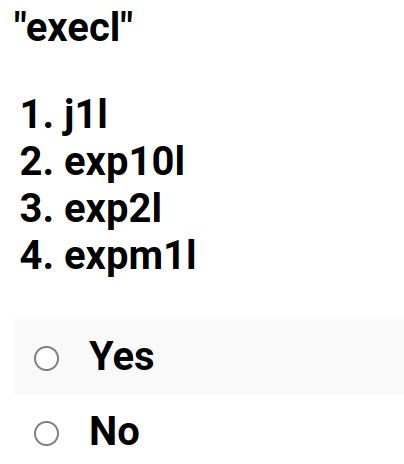
\includegraphics[scale=0.2]{pictures/survey-example-negative.png}
          \caption{Positve exmaple}
      \end{minipage}
      \begin{minipage}{0.45\textwidth}
          \centering
          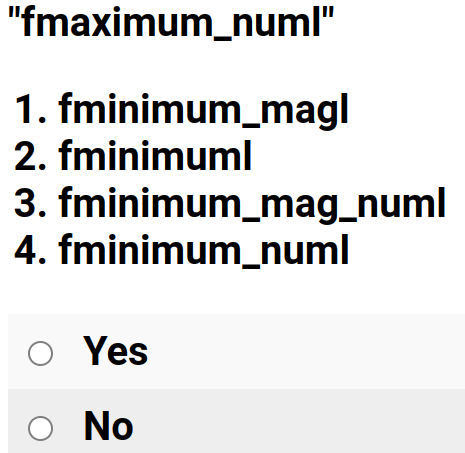
\includegraphics[scale=0.2]{survey-example-positive.png}
          \caption{Negative exmaple}
      \end{minipage}
      \begin{table}
        \begin{center}
          \scalebox{0.8} {
            \begin{tabular}{ |p{1.5cm}||p{4.5cm}|p{3.2cm}|p{4cm}|p{1.8cm}|  }
            \hline
            \multicolumn{5}{|c|}{Ergebnisse der Expertenbefragung} \\
            \hline
            Strategie & Code-Llama-Erklärungen & Funktionsnamen & Funktionskommentare & \textit{Code2Vec} \\
            \hline
            Score   & 0.596 & 0.532 & 0.433 & 0.321   \\
            \hline
            \end{tabular}
          }
        \end{center} 
      \end{table}
    \end{figure}
\end{frame}
\begin{frame}[t]{Embeddings space comparison}
\end{frame}
\begin{frame}[t]{Embeddings space comparison}
\end{frame}
\begin{frame}[t]{Evaluation with T-SNE}
\end{frame}

\section{Limitations}
\begin{frame}
  HALLO
\end{frame}

\section{Conclusion \& Future Work}
\begin{frame}
  HALLO
\end{frame}

\appendix

\begin{frame}{Discussion}
\end{frame}

\end{document}

\begin{frame}
  \vspace{0.4cm}
  \centering
  
\includegraphics[scale=0.12]{lmu-logo.png}
  \titlepage
\end{frame}
